\graphicspath{{fig/model_development/}}

\chapter{Model Development}
\label{cha:model_dev}

In this chapter we shall introduce one of the most popular and well studied agent-based
models in the literature: the Vicsek model. The Vicsek model represents a simple alignment
model in which agents interact with neighbours within some given distance. Despite its
simplicity, this model can produce sophisticated dynamics reminiscent of real flocking
events. A phase transition from order to disorder is observed as the amount of noise in
the model is regulated.

The Vicsek model, like many other ABMs, implements a discontinuous interaction rule. With
this the onset of interaction between individuals is very sensitive to small perturbations
in distances. We consider continuous interaction rules as a biologically-motivated
alternative. Such rules ensure interactions are more robust to small perturbations in
distances, but without the penalty of additional model complexity.

\section{The Vicsek Model}

The Vicsek model simulates the movements of $N$ individuals moving with constant speed
$v$. All movement takes place in a square-cell with periodic boundary conditions and side
length $L$. To initialise a simulation agents are allocated a random position within
the cell, and a random direction of motion. From time $t$ to time $t+1$ agent $i$ updates
its position as:
\begin{equation*}
    \bm{x}_{i, t+1} = \bm{x}_{i, t} + \bm{v}_{i, t},
\end{equation*}
where the velocity $\bm{v}_{i,t}$ is constructed to have speed $v$ and direction of motion
$\theta_{i, t+1}$. Updating $\theta_{i,t}$ to $\theta_{i, t+1}$ models how agents update
their directions of motion in light of their neighbours' movements. The ability of
individuals to observe and react to the movements of their neighbours is assumed to be
imperfect, and so a noise term, in the form of a random directional perturbation, is
introduced. In the Vicsek model noise is considered to be uniformly distributed as
$\mathcal{U}(-\eta/2, \eta/2)$. The directional update of agent $i$ can then be expressed
as:
\begin{equation}
    \label{eq:vicsek_update}
    \theta_{i, t+1} \given \angmean{\theta}_{i, t}, \eta \sim
                     \mathcal{U}(\angmean{\theta}_{i, t} - \eta/2,
                                 \angmean{\theta}_{i, t} + \eta/2),
\end{equation}
where $\angmean{\theta}_{i, t}$ represents the average direction of motion of agent $i$'s
neighbours at time $t$. The computation of $\angmean{\theta}_{i, t}$ is described by a
weighted circular mean:
\begin{equation}
    \angmean{\theta}_{i, t+1} = \atantwo\bigg(
        \sum_{j=1}^N \omega_{ij, t} \sin\theta_{j,t},
        \sum_{j=1}^N \omega_{ij, t} \cos\theta_{j,t}
    \bigg).
\end{equation}
With this, the weighting $\omega_{ij, t}$ represents the strength of the interaction
between agent $i$ and agent $j$ at time $t$. In the Vicsek model agent $i$ interacts
with neighbours which are within distance $r$ of its current position. This interaction
can be implemented with the weighting rule
\begin{equation}
    \label{eq:vicsek_interaction}
    \omega_{ij,t} =
    \begin{cases}
        1 & \text{ if } d_{ij, t} \leq r,\\
        0 & \text{ otherwise,}
    \end{cases}
\end{equation}
where $d_{ij,t}$ is the Euclidean-distance between the positions of agent $i$ and agent
$j$ at time $t$:
\begin{equation*}
    d_{ij,t} = \sqrt{(x_{j,t} - x_{i,t})^2 + (y_{j,t} - y_{i,t})^2}.
\end{equation*}

The interaction rule implemented in the Vicsek model represents a discontinuous
interaction, as the interaction kernel is very sensitive to small perturbations in
distances.  More formally, this discontinuity can be shown by considering the value of
$\omega_{ij, t}$ as $d_{ij,t}$ tends to $r$ from above and below. As $d_{ij,t}$ tends to
$r$ from above we realise $\lim_{d_{ij,t} \rightarrow r^+} \omega_{ij,t} = 0$.
Conversely, as $d_{ij,t}$ tends to $r$ from below we observe: $\lim_{d_{ij,t} \rightarrow
r^-} \omega_{ij,t} = 1$. As the weighting tends to different values as the limit of
$d_{ij,t}=r$ is approached from above and below we see that this weighting rule exhibits a
discontinuity.

The Vicsek model was motivated by considering models for ferromagnetism. In these models
particles align spin states with neighbouring particles. Although a discontinuous
interaction rule may be appropriate for such models, it is not clear whether the
hard cut-off imposed by the interaction radius is appropriate for biological systems.

To quantify the polarisation of a flock at time $t$ Vicsek considered the absolute value
of the normalised velocity of a flock:
\begin{equation}
    v_{a,t} = \frac{1}{Nv} \abs{\,\sum_{i=1}^N \bm{v}_{i,t}\,}.
\end{equation}
A flock in which
agents are directed randomly, and not moving in any cohesive manner at time $t$, exhibit
$v_{a,t}\approx0$. Conversely, a highly polarised flock in which all members are moving in
the same direction at time $t$ have an alignment $v_{a,t}=1$.

\begin{figure}[tb]
    \begin{subfigure}[b]{0.5\textwidth}
        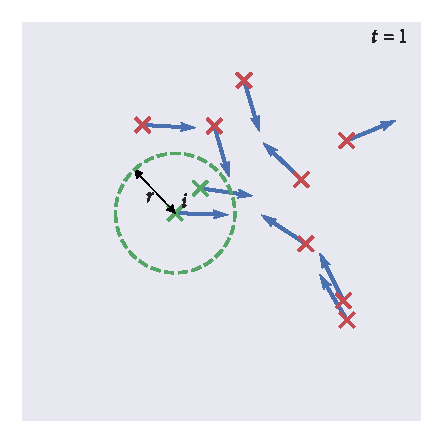
\includegraphics{vicsek_simulation_1.pdf}
    \end{subfigure}%
    \begin{subfigure}[b]{0.5\textwidth}
        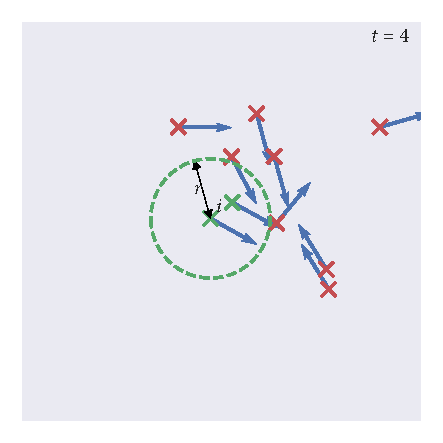
\includegraphics{vicsek_simulation_4.pdf}
    \end{subfigure}
    \begin{subfigure}[b]{0.5\textwidth}
        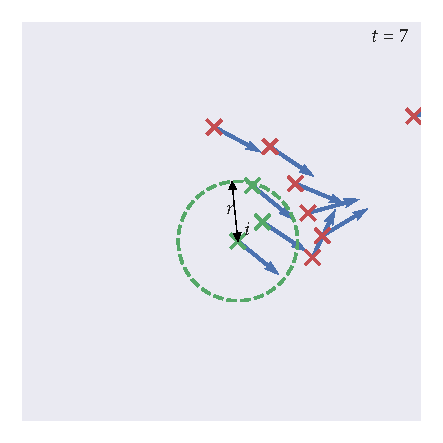
\includegraphics{vicsek_simulation_7.pdf}
    \end{subfigure}%
    \begin{subfigure}[b]{0.5\textwidth}
        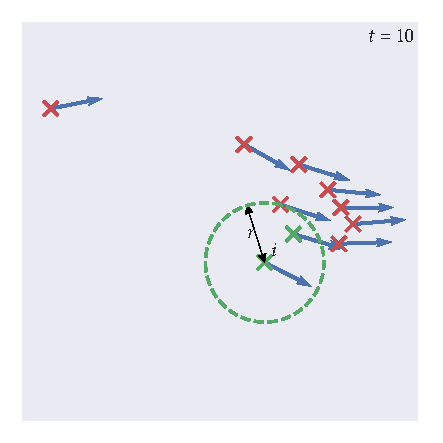
\includegraphics{vicsek_simulation_10.pdf}
    \end{subfigure}
    \caption{Visualisations from a simulation of the Vicsek model. At time $t=1$, $N=10$
        agents are assigned random positions within a square-cell of side length $L=1$.
        Initially, the directions of motion of individuals are realised from a
        $\mathcal{U}(-\pi, \pi)$ distribution. Between time steps agents move with speed
        $v=0.03$, and update directions according to \cref{eq:vicsek_update}, with
        $\eta=\pi/16$. The interaction zone of agent $i$ is illustrated throughout the
        simulation by a circle of radius $r$ centred at $\bm{x}_{i,t}$. The positions of
        neighbours within agent $i$'s interaction zone are visualised with a green cross.
        Individuals which lie outside of agent $i$'s interaction zone have their positions
        denoted by a red cross.}
\end{figure}

\subsection{Considerations of stochasticity}

Inspired by models of interacting particles, the uniformly distributed noise implemented in
simulations of the Vicsek model is analogous to temperature in a physical system. However,
it is not clear whether this distribution is a reasonable choice for biologically-motivated
systems. In much of the literature authors instead assume that noise is normally
distributed. In this case an agent's directional update typically takes the form:
\begin{equation*}
    \theta_{i,t+1} \given \angmean{\theta}_{i,t}, \sigma_Y \sim
        \mathcal{N}(\angmean{\theta}_{i,t}, \sigma_Y).
\end{equation*}

Throughout this work we shall also consider the possibility that the noise experienced by
individuals is distributed according to some generalised Student's $t$-distribution with
$\nu$ degrees of freedom. In this situation, the directional update of agent $i$ would
then be expressed as:
\begin{equation*}
    \theta_{i,t+1} \given \angmean{\theta}_{i,t}, \nu, \sigma_Y \sim
    t_{\nu}(\angmean{\theta}_{i,t}, \sigma_Y).
\end{equation*}
The Student's $t$-distribution allows more weight in its tails than the normal
distribution permits. However, as $\nu\rightarrow\infty$ the Student's $t$-distribution
with location $\mu$ and scale $\sigma_Y$ converges to a normal distribution with mean and
standard deviation corresponding to these location and scale parameters.  Although the
Student's $t$-distribution represents a more flexible noise structure, it also comes at
the cost of model complexity: with the introduction of the degrees of freedom as an
additional model parameter.

\subsection{Boundary conditions \& trajectory plots}

Recall that all simulations of the Vicsek model take place in a square-cell with periodic
boundary conditions and side-length $L$. In this way the density of the cell remains
constant throughout a simulation. However, implementing periodic boundary conditions when
we attempt to mimic real flocking events is clearly inappropriate. Instead, we shall
consider simulations to take place in the unrestricted continuous domain represented by
$\mathbb{R}^2$.  On top of realism, performing simulations in this unrestricted domain
allows more informative visualisations of the resulting data, as in
\cref{fig:example_traj}.
\begin{figure}[tb]
    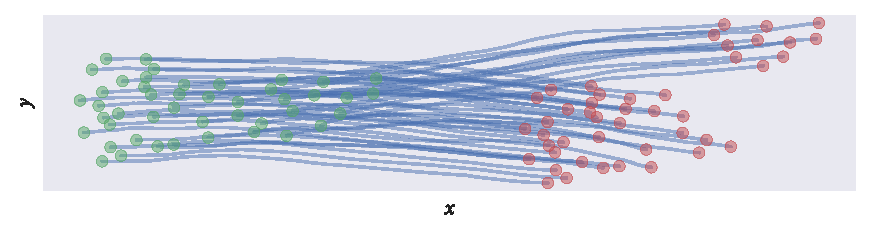
\includegraphics{example_traj_plot.pdf}
    \caption{A trajectory plot representing the movements of $N=45$ agents moving through
        the unrestricted continuous domain $\mathbb{R}^2$. Agents are initially positioned
        at the locations represented by the green markers. The model is simulated for
        $200$ time steps. The red markers represent the positions of agents at the end of
        a simulation. Blue lines represent the trajectories of motion of individual agents
        throughout the simulation.}
    \label{fig:example_traj}
\end{figure}

\section{Continuous interaction models}

It has been seen that the interaction rule implemented in the Vicsek model exhibits a
discontinuity. This discontinuity represents two concerns for the authors. Firstly, the
biological realism of an interaction rule implementing a hard cut-off is brought into
question. Secondly, the ability to fit such a model to data is seen to be potentially
problematic: effectively exploring the sample space of a discontinuous target
distribution can be difficult.

Such concerns can be addressed by considering variations of the Vicsek model in which
continuous interaction rules are implemented. The authors consider that such rules may
represent more biologically realistic behaviours. In addition to this, effective
parameter inference on models with these rules is expected to be more attainable.

\subsection{Metric models}

\subsection{Topological models}
